\documentclass{bmstu}

\bibliography{biblio}

\usepackage{listings}
\usepackage{rotating}

\usepackage{pdfpages}




\begin{document}

\renewcommand\labelitemi{---}

% \makecourseworktitle{Информатика, искусственный интеллект и системы управления}{Программное обеспечение ЭВМ и информационные технологии}{Разработка базы данных приложения бронирования студий}{Турчанский~Н.~А./ИУ7-64Б}{Исаев~А.~Л.}{}{}{}


\includepdf[pages=1]{title.pdf}

\chapter*{РЕФЕРАТ}
\b{Ключевые слова}
Роль музыки в структуре духовной жизни современного человека довольно велика, а музыкальная культура в целом становится значительным фактором формирования общечеловеческих ценностей \cite{music_for_youth}.
Современные технологии дали возможность не только прослушивать композиции через электронные устройства, но и записывать их, а специально оборудованные студии помогают облегчить этот процесс.

Цель курсовой работы --- разработка базы данных приложения бронирования студий.
Для достижения поставленной цели необходимо выполнить следующие задачи:

\begin{enumerate}
	\item провести анализ предметной области;
	\item выполнить формализацию задачи;
	\item сформулировать описание пользователей;
	\item спроектировать сущности базы данных;
	\item выбрать средства реализации базы данных и приложения;
	\item разработать базу данных и приложение;
	\item провести исследование зависимости времени от сложности запроса.
\end{enumerate}

\maketableofcontents

\begin{definitions}
	\definition{База данных}{это совокупность данных, оргаизованных по определенным правилам, предусматривающим общие принципы описания, хранения и манипулирования данными, независимая от прикладных программ \cite{data_base}.}
	\definition{Система управления базами данных}{это программное обеспечение для создания и редактирования баз данных, просмотра и поиска информации в них \cite{dbms}.}
\end{definitions}
\begin{abbreviations}
	\definition{БД}{База Данных}
	\definition{СУБД}{Система Управления Базами Данных}
	\definition{SQL}{Structed Query Language}
\end{abbreviations}


\chapter*{ВВЕДЕНИЕ}
\addcontentsline{toc}{chapter}{ВВЕДЕНИЕ}
Музыка играет важную роль в жизни современного человека и в значительной степени влияет на формирование общечеловеческих ценностей~\cite{music_for_youth}.
Современные технологии дали возможность не только прослушивать композиции через электронные устройства, но и записывать их, а специально оборудованные студии помогают облегчить этот процесс.

Цель курсовой работы --- разработка базы данных приложения бронирования студий.
Для достижения поставленной цели необходимо выполнить следующие задачи:

\begin{enumerate}
	\item провести анализ предметной области;
	\item выполнить формализацию задачи;
	\item сформулировать описание пользователей;
	\item спроектировать сущности базы данных;
	\item выбрать средства реализации базы данных и приложения;
	\item разработать базу данных и приложение;
	\item провести исследование зависимости времени от сложности запроса.
\end{enumerate}

\chapter{Аналитический раздел}
В данном разделе будет представлен анализ предметной области, проведена формализация задачи, проведена формализация и описание информации для хранения в БД, проведена формализация и описание пользователей и проанализированы модели баз данных. 
\section{Анализ предметной области}
Развитие информационных технологий, помимо различных сфер по всей земле, также не обошло и музыкальную сферу.
Музыкальная индустрия одной из первых ощутила на себе смену технологических эпох, изменившись за последние 20 лет на всех уровнях \cite{music_and_it}.

Российский рынок услуг звукозаписи --- это динамично развивающаяся отрасль, которая с каждым годом приобретает все большую популярность и значимость.
Еще в 2017 году в России было примерно 656 студий звукозаписи, а в 2023 году их насчитывалось около 1160 студий звукозаписи и репетиционных точек \cite{music_stat}.

%\includeimage
%{stat} % Имя файла без расширения (файл должен быть расположен в директории inc/img/)
%{n} % Обтекание (с обтеканием)
%{c} % Положение рисунка (см. wrapfigure из пакета wrapfig)
%{0.33\textwidth} % Ширина рисунка
%{Tuz} % Подпись рисунка

\begin{center}
	\centering
	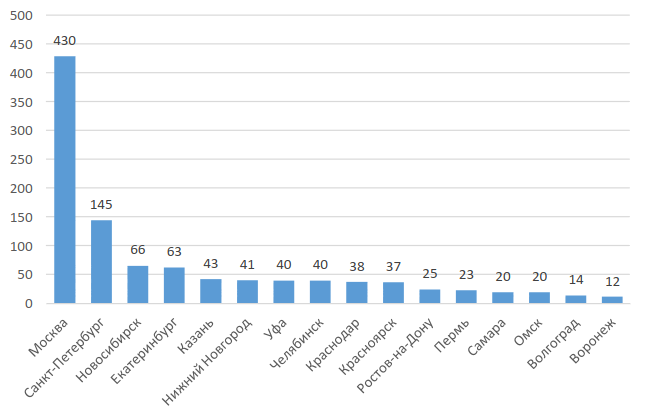
\includegraphics[height=0.3\textheight]{inc/img/stat.png}
	\captionof{figure}{Количество студий звукозаписи на момент 20.04.2023 \cite{music_stat}}
	\label{img:stat}
\end{center}


В связи с этим, онлайн бронирование в студии звукозаписи приобрели весомое значение в нынешнее время.

\section{Формализация задачи}
Для выполнения поставленной цели необходимо разработать БД для хранения информации о студиях, об их составляющем, о пользователях и о бронях, которые пользователи создают.

Также необходимо спроектировать и разработать приложение, которое будет предоставлять интерфейс для работы с БД и давать возможность для каждого авторизованного пользователя создавать бронь на определенное время, резервируя комнату, оборудование, продюсера и инструменталиста.

Нужно предусмотреть возможность добавления, изменение и удаление студий, комнат, оборудования, продюсеров и инструменталистов.
Необходимо реализовать разный функционал для разных категорий пользователей.

\section{Формализация и описание информации, подлежащей хранению в БД}
Разрабатываемая БД для приложения бронирования студий должна содержать информацию:
\begin{itemize}
	\item о зарегистрированных пользователях;
	\item об имеющихся студиях;
	\item о комнатах, принадлежащих студиям;
	\item об оборудовании, принадлежащем студиям;
	\item о продюсерах, работающих на студиях;
	\item об инструменталистах, работающих на студиях;
	\item о бронях на выбранное время на определенную комнату, оборудование, продюсера и инструменталиста.
\end{itemize}

На рисунке \ref{img:er} представлена ER--диаграмма сущностей в нотации Чена.

\begin{center}
	\centering
	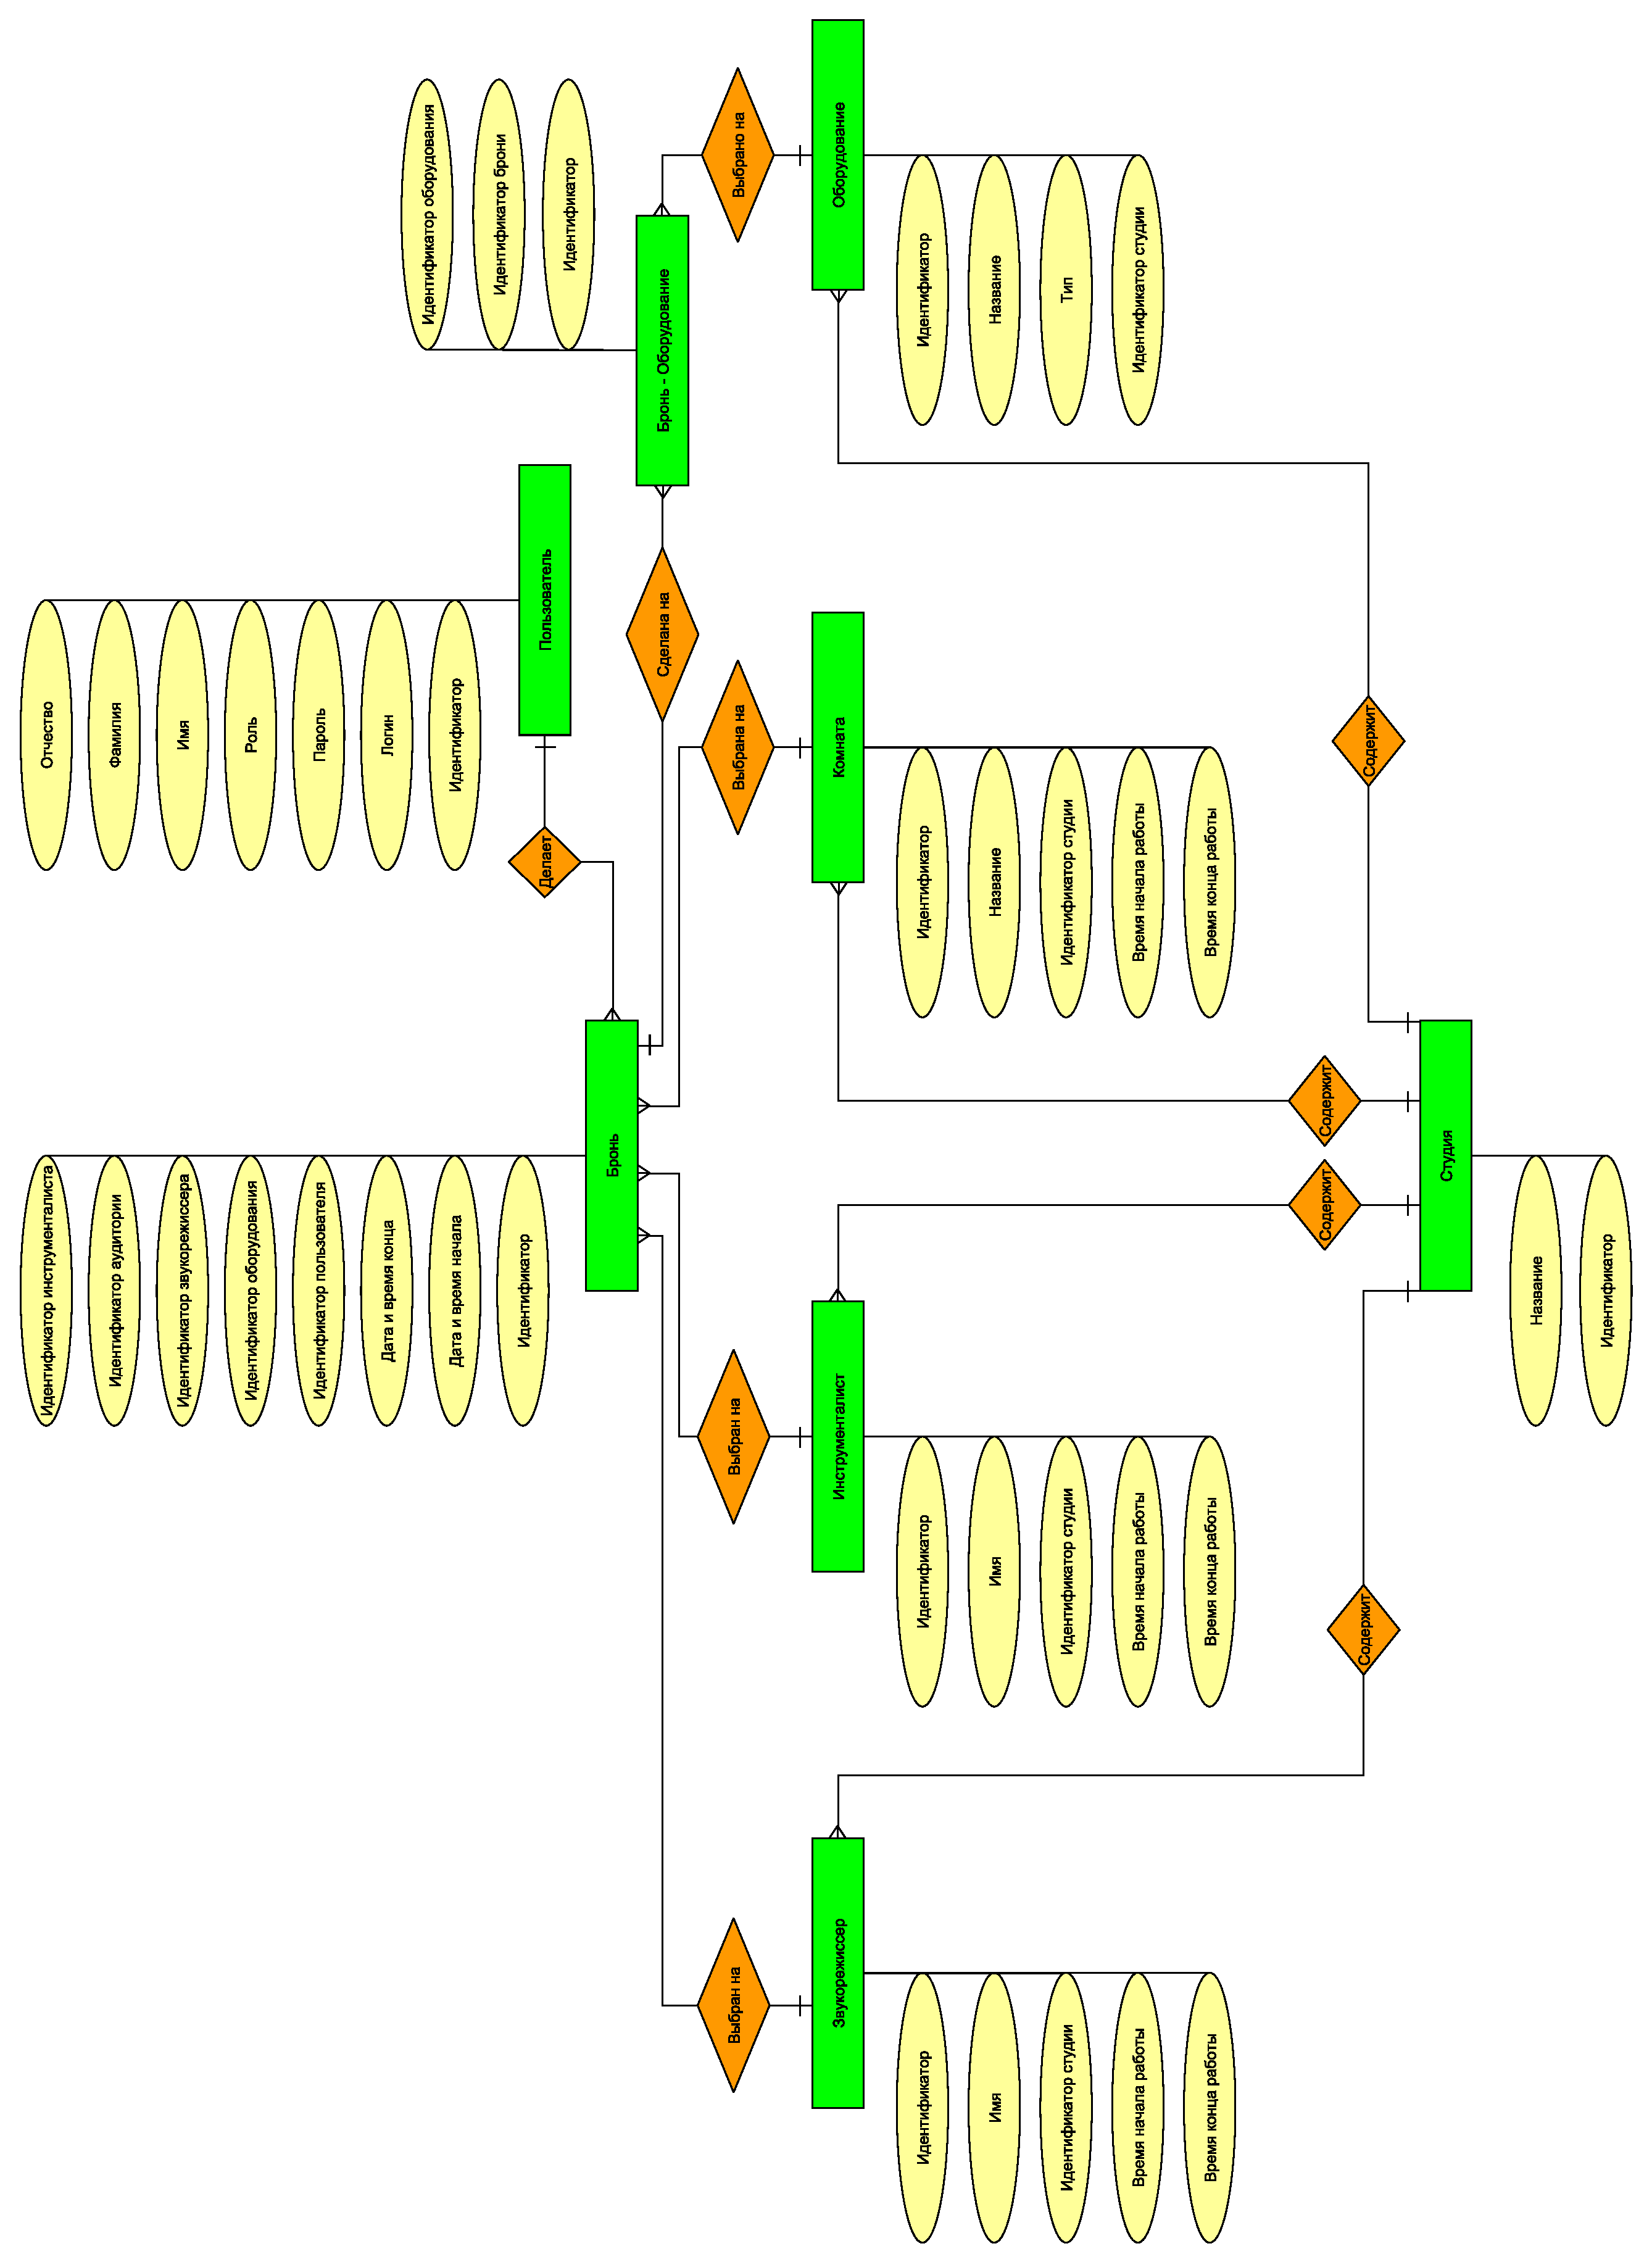
\includegraphics[height=0.9\textheight]{inc/img/er_90.pdf}
	\captionof{figure}{ER--диаграмма}
	\label{img:er}
\end{center}

\section{Формализация и описание пользователей проектируемого приложения в БД}
Для взаимодействия с приложением было выделено три категории пользователей:
\begin{enumerate}
	\item гость;
	\item авторизованный пользователь;
	\item администратор.
\end{enumerate}

Гость имеет право воспользоваться только начальным функционалом приложения: просмотром броней, регистрацией и входом в аккаунт.
При успешном прохождении авторизации пользователь автоматически становится авторизованным пользователем.

Функционал авторизованного пользователя является более расширенным и включает в себя: создание, просмотр и отмена уже созданных броней. 
Также есть возможность изменение личных данных, выхода из профиля и выхода из приложения.

Если пользователь войдет под именем администратора, то он будет иметь возможность:
\begin{itemize}
	\item добавления, изменения и удаления студий;
	\item добавления, изменения и удаления комнат;
	\item добавления, изменения и удаления оборудования;
	\item добавления, изменения и удаления продюсеров;
	\item добавления, изменения и удаления инструменталистов.
\end{itemize}
		
На рисунке \ref{img:use_case} представлены пользовательские сценарии.

\begin{center}
	\centering
	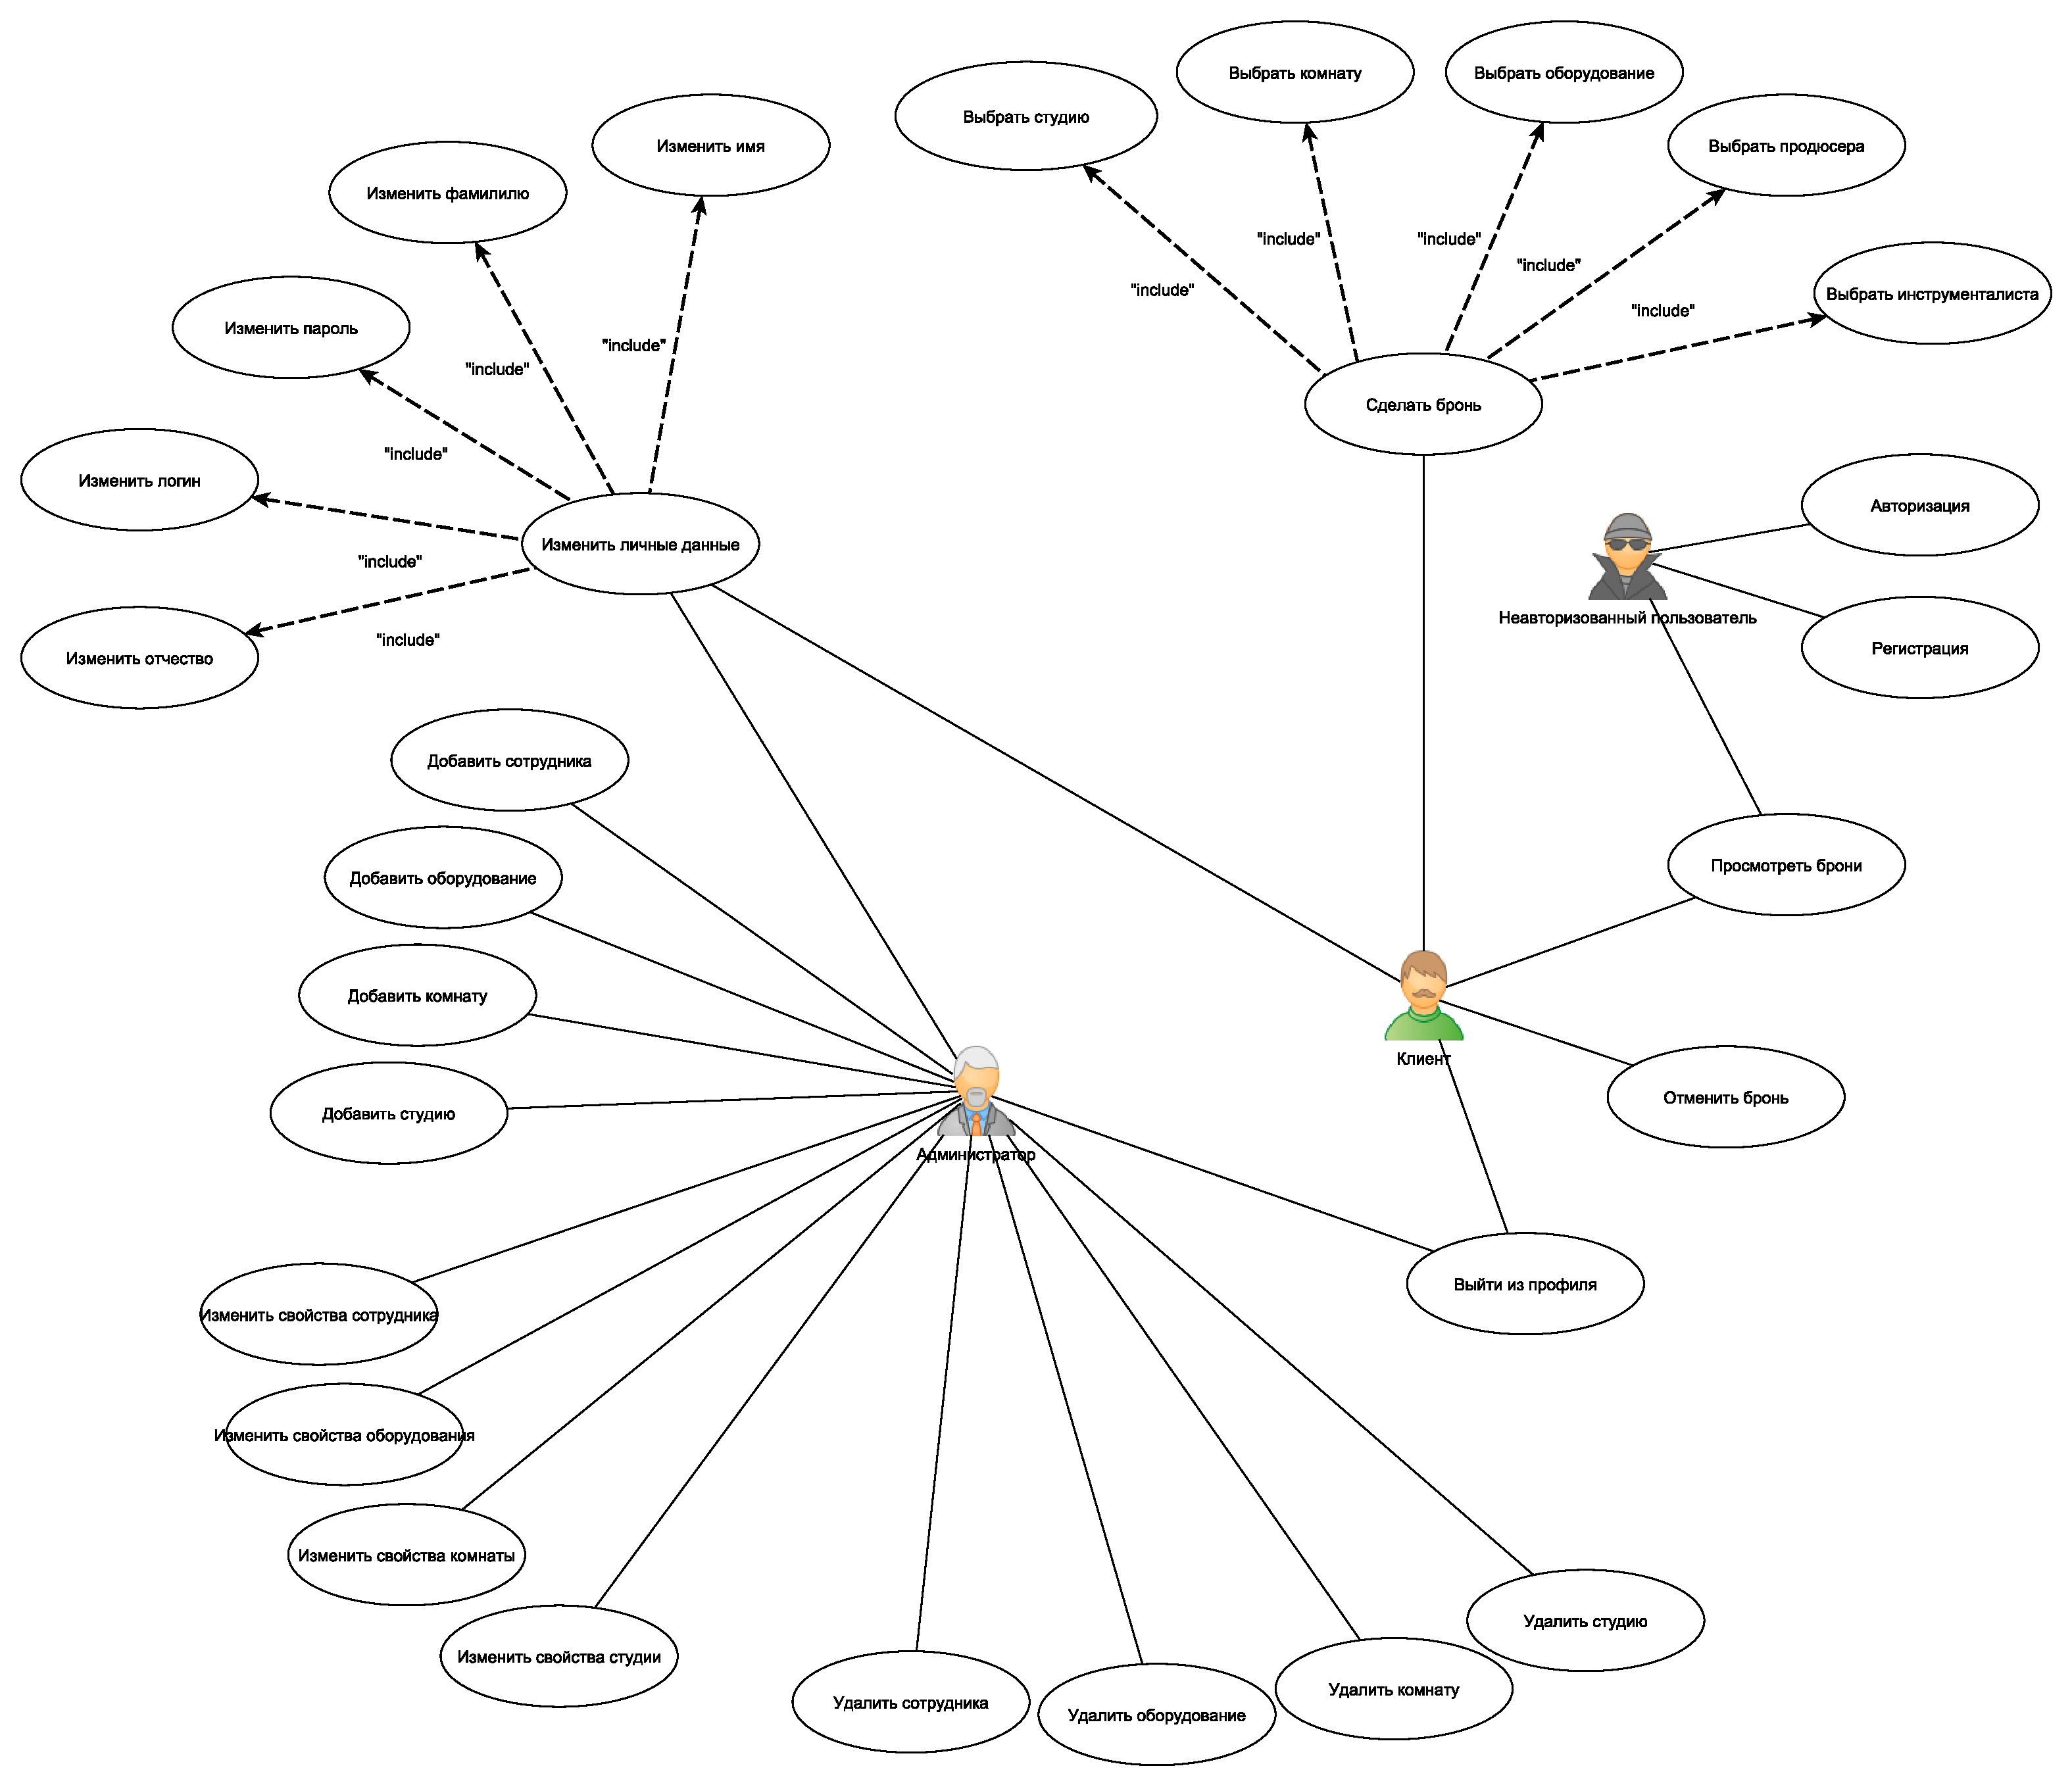
\includegraphics[height=0.55\textheight]{inc/img/use_case.pdf}
	\captionof{figure}{Пользовательские сценарии}
	\label{img:use_case}
\end{center}

% В рамках данной работы необходимо разработать веб приложение, 


\section{Анализ существующих баз данных}
Базы данных по способу хранения делят на две группы --- колоночные и строковые.

\subsection{Колоночные базы данных}
В колоночных базах данных значения одного атрибута хранятся последовательно друг за другом.
Каждая колонка, хранимая на диске, разделена на блоки определенного размера.
Блок состоит из заголовка, размер которого пренебрежительно мал по сравнению с размером блока и непосредственно данных.
Каждой записи в столбце сопоставляется ее позиция (номер строки) \cite{strokovie_and_kolonochnie_bd}.
\subsection{Строчные базы данных}
Под строчным хранением данных обычно понимается физическое хранение кортежа любого отношения в виде одной записи, в котором значение атрибута идут последовательно одно за другим, а за последним атрибутом кортежа в общем случае следует новый кортеж отношения.
План запроса представляет собой дерево, у каждого узла которого имеется один родитель и один (или два в случае пересечения) дочерних узла
\cite{strokovie_and_kolonochnie_bd}.



\section{Анализ моделей баз данных}
Модель данных --- совокупность структур данных и операций по их обработке \cite{dbms}.

Существуют модели данных следующих типов:
\begin{itemize}
	\item дореляционные;
	\item реляционные;
	\item постреляционные.
\end{itemize}

\subsection{Дореляционные модели}
К дореляционным моделям относят модель инвертированных списков, иерархическую модель и сетевую модель:

\begin{enumerate}
	\item модель инвертированных списков.
	БД на основе модели инвертированных списков представляет собой совокупность файлов, содержащих записи.
	Для записей в файле определен некоторый порядок, диктуемый физический организацией данных.
	Для каждого файла может быть определено произвольное число других упорядоченностей на основании значений некоторых полей записей.
	Обычно для этого используются индексы.
	В такой модели данных отсутствуют ограничения целостности как таковые.
	Все ограничения на возможные экземпляры БД задаются теми программами, которые работают с БД.
	Одно из немногих ограничений, которое может присутствовать --- это ограничение, задаваемое уникальным индексом;
	
	\item иерархическая модель данных строится по принципу иерархии типов объектов, то есть один из типов объекта является главным, а остальные, находящиеся на низших уровнях иерархии, --- подчиненными.
	Между главным и подчиненными объектами устанавливается взаимосвязь <<один~--~ко~--~многим>> \cite{dbms};
	
	\item В сетевой модели данных любой объект может быть и главным, и подчиненным.
	Один и тот же объект может одновременно выступать и в роли владельца, и в роли члена набора.
	Это означает, что любой объект может участвовать в любом числе зависимостей \cite{dbms}.
\end{enumerate}

\subsection{Реляционные модели}
База данных на реляционной модели представляет собой множество отношений.
Множество отношений и операций над ними образуют реляционную алгебру.
Список операций содержит проекцию, выборку, объединение, пересечение, вычитание, соединение и деление \cite{dbms}.

\subsection{Постреляционные модели}
Классическая реляционная модель предполагает неделимость данных, хранящихся в полях записей таблиц.
Это означает, что информация в таблице представляется в первой нормальной форме.
Существует ряд случаев, когда это ограничение мешает эффективной реализации приложений.
Постреляционная модель данных представляет собой расширенную реляционную модель, снимающую ограничение неделимости данных, хранящихся в записях таблиц.
Постреляционная модель данных допускает многозначные поля --- поля, значения которых состоят из подзначений.
Набор значений многозначных полей считается самостоятельной таблицей, встроенной в основную таблицу \cite{voroneg}.
 
\section*{Вывод}
В данном разделе была проанализирована предметная область, проведена формализация задачи, проведена формализация и описание информации, проведена формализация и описание пользователей и проанализированы модели баз данных. 

% \section{Анализ систем управления базами данных}
 
 % про субд https://cyberleninka.ru/article/n/obosnovanie-vybora-modeli-hraneniya-dannyh-dlya-sistemy-monitoringa-kosmicheskogo-prostranstva/viewer
\chapter{Конструкторский раздел}

В данном разделе будет представлена диаграмма проектируемой БД, описание сущностей, описание проектируемой ролевой модели и описание проектируемых процедур.

\section{Диаграмма проектируемой базы даннызх}
На рисунке~\ref{img:db} изображена диаграмма проектируемой базы данных.

\begin{center}
	\centering
	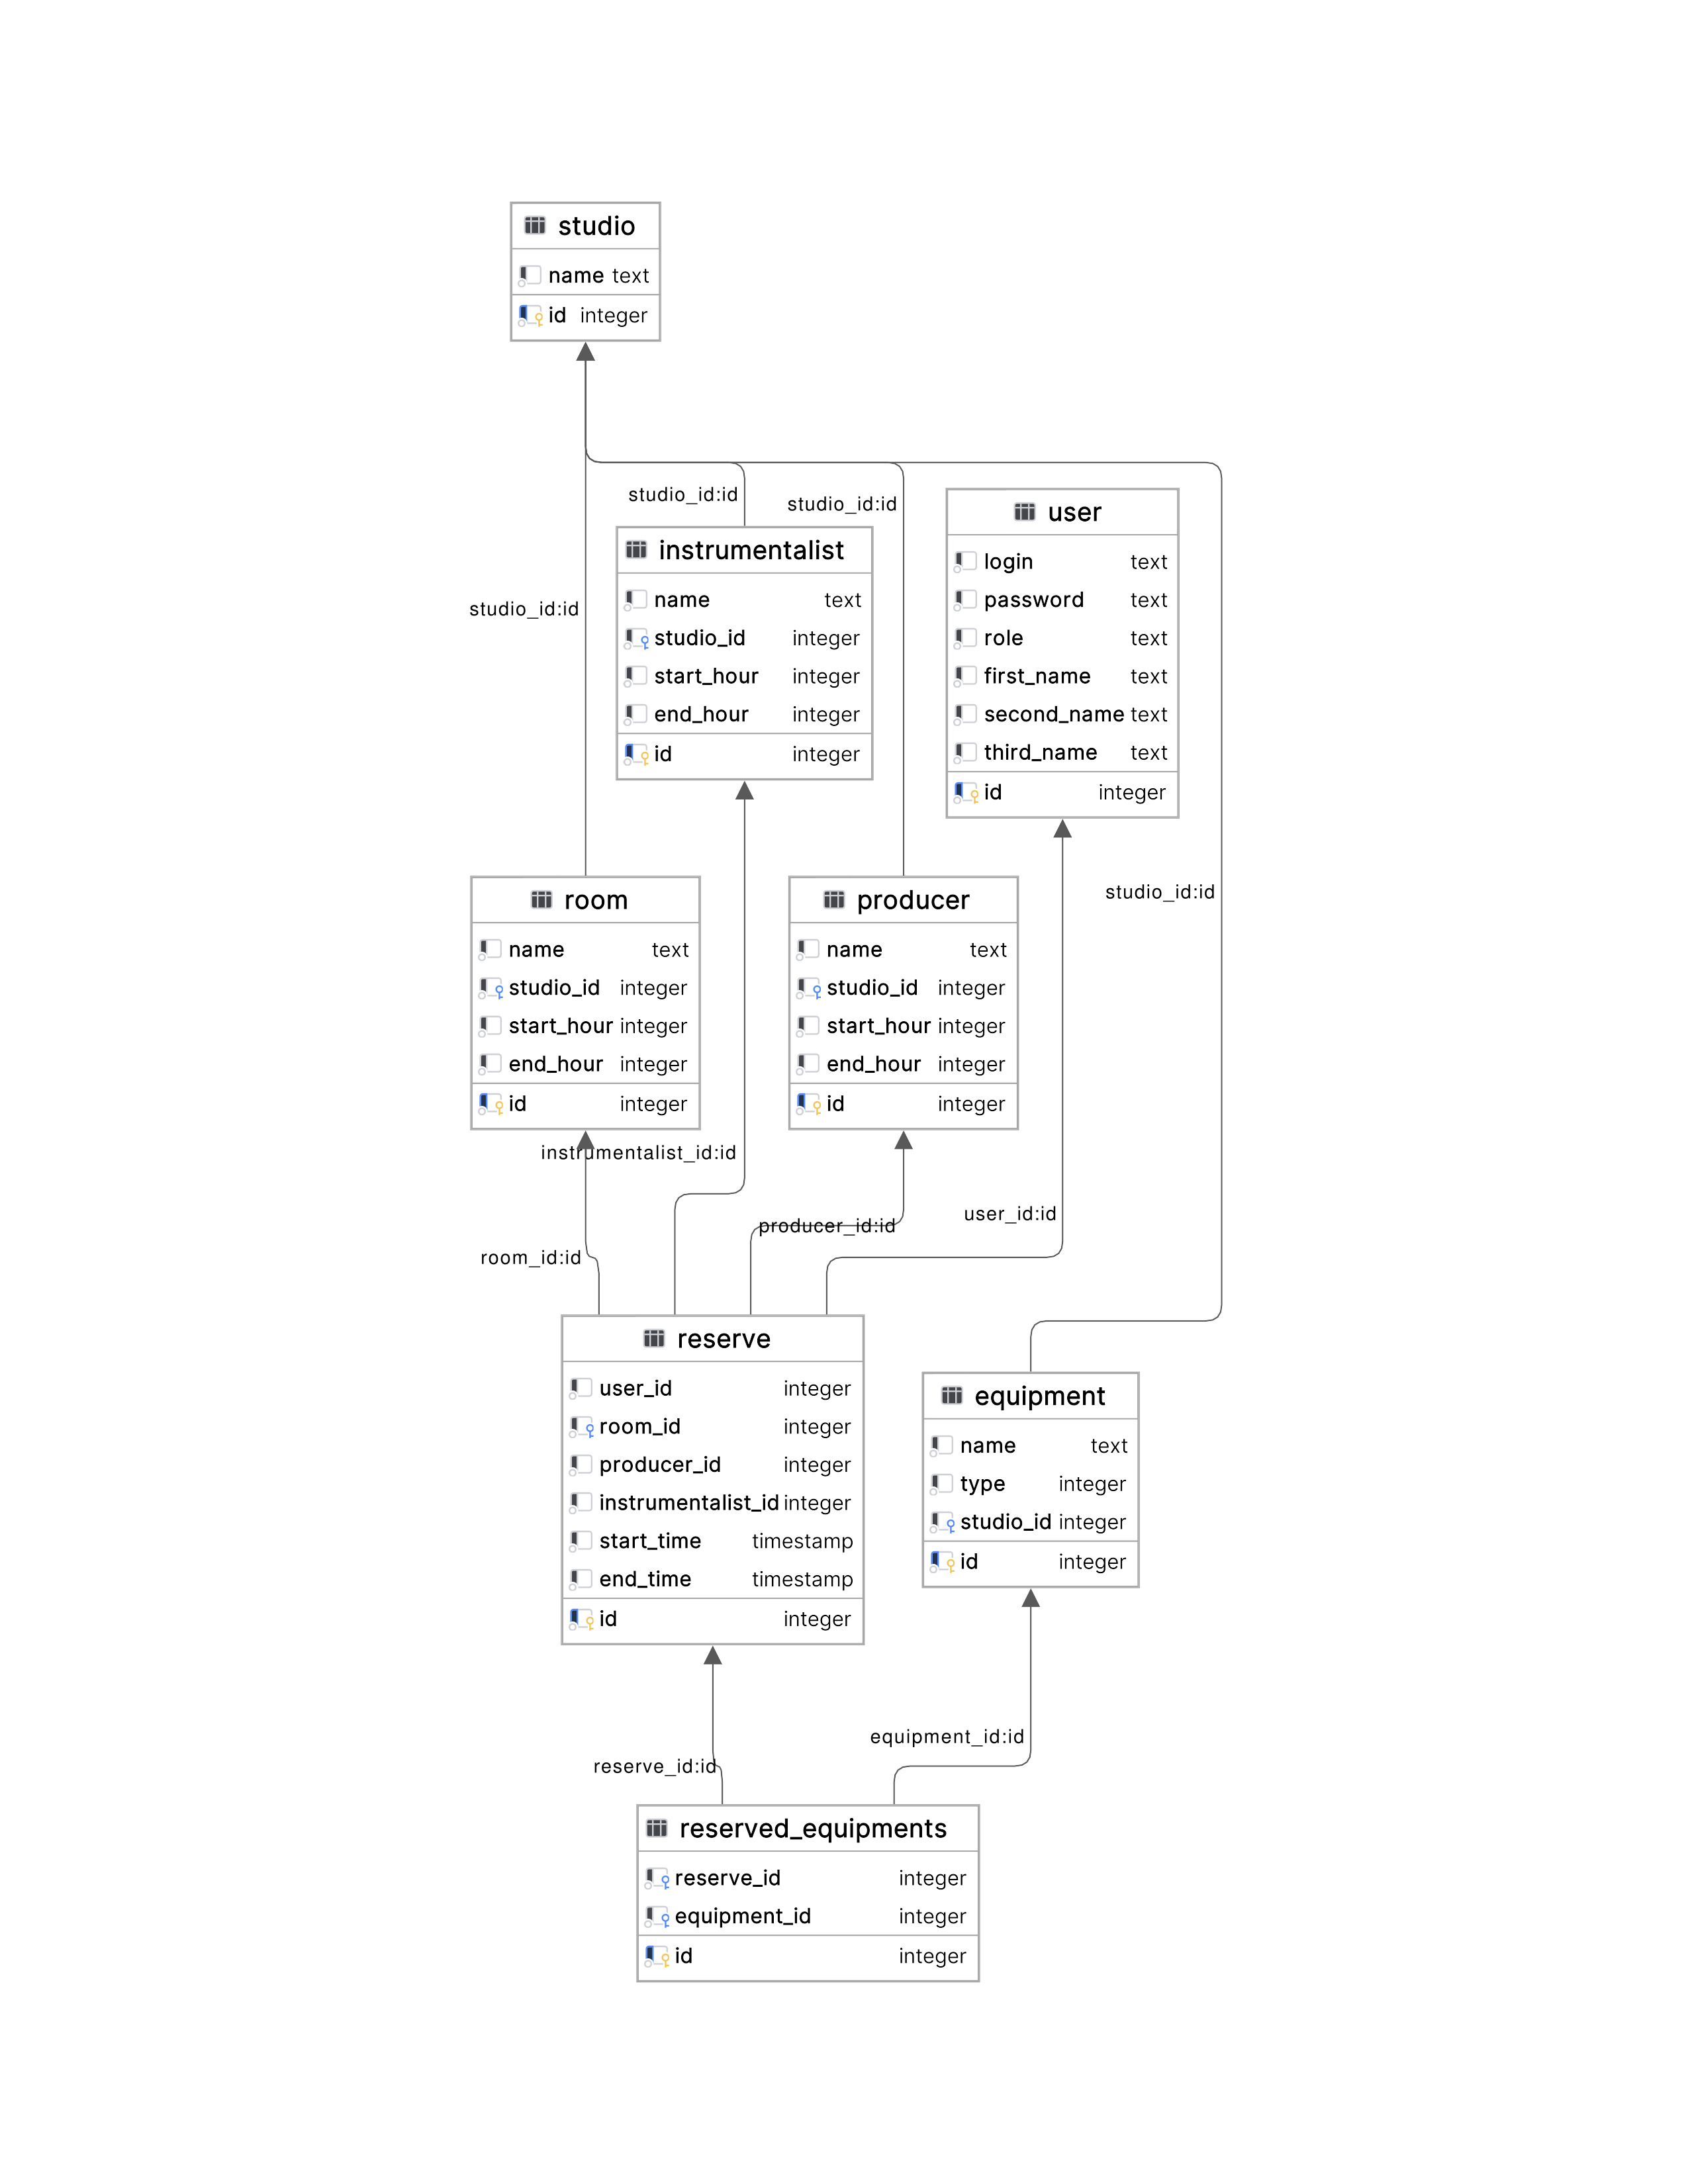
\includegraphics[height=0.83\textheight]{inc/img/public}
	\captionof{figure}{Диаграмма базы данных}
	\label{img:db}
\end{center}
\section{Описание сущностей}
База данных будет спроектирована из следующих сущностей:
\begin{enumerate}
	\item таблица \textit{User}, в которой хранятся данные об пользователях;
	\item таблица \textit{Reserve}, в которой хранятся данные об бронях;
	\item таблица \textit{Studio}, в которой хранятся данные об студиях;
	\item таблица \textit{Room}, в которой хранятся данные об комнатах студий;
	\item таблица \textit{Equipment}, в которой хранятся данные об оборудовании;
	\item таблица \textit{Reserved\_equipment}, в которой хранятся данные об зарезервированном оборудовании;
	\item таблица \textit{Producer}, в которой хранятся данные об звукорежиссерах студий;
	\item таблица \textit{Instrumentlist}, в которой хранятся данные об инструменталистах студий.
\end{enumerate}
\subsection{Таблица User}
Таблица \textit{User} содержит информацию об идентификаторе пользователя, логине, пароле, роле, имени, фамилии и отчестве.
Имеет следующие атрибуты:
\begin{itemize}
	\item \textit{id} --- целое число, первичный ключ, идентификатор пользователя;
	\item \textit{login} --- строка, логин пользователя;
	\item \textit{password} --- строка, пароль пользователя;
	\item \textit{role} --- целое число, роль пользователя;
	\item \textit{first\_name} --- строка, имя пользователя;
	\item \textit{second\_name} --- строка, фамилия пользователя;
	\item \textit{third\_name} --- строка, отчество пользователя.
\end{itemize}
\subsection{Таблица Reserve}
Таблица \textit{Reserve} содержит информацию об идентификаторе брони, идентификаторе пользователя, идентификаторе комнаты, идентификаторе продюссера, идентификаторе инструменталиста, время начала брони, время конца.
Имеет следующие атрибуты:
\begin{itemize}
	\item \textit{id} --- целое число, первичный ключ, идентификатор брони;
	\item \textit{user\_id} --- целое число, внешний ключ, идентификатор пользователя;
	\item \textit{room\_id} --- целое число, внешний ключ, идентификатор комнаты;
	\item \textit{producer\_id} --- целое число, внешний ключ, идентификатор продюссера;
	\item \textit{instrumentalist\_id} --- целое число, внешний ключ, идентификатор инструменталиста;
	\item \textit{start\_time} --- тип хранения даты и времени, время начала брони;
	\item \textit{end\_time} --- тип хранения даты и времени, время конца брони.
\end{itemize}
\subsection{Таблица Studio}
Таблица \textit{Studio} содержит информацию об идентификаторе студии и названии студии.
Имеет следующие атрибуты:
\begin{itemize}
	\item \textit{id} --- целое число, первичный ключ, идентификатор студии;
	\item \textit{name} --- строка, название студии.
\end{itemize}
\subsection{Таблица Room}
Таблица \textit{Room} содержит информацию об идентификаторе комнаты, названии комнат, идентификаторе студии (к которой принадлежит оборудование), времени начала работы комнаты и времени конца работы комнаты.
Имеет следующие атрибуты:
\begin{itemize}
	\item \textit{id} --- целое число, первичный ключ, идентификатор комнаты;
	\item \textit{name} --- строка, название комнаты;
	\item \textit{studio\_id} --- целое число, внешний ключ, идентификатор студии;
	\item \textit{start\_time} --- тип хранения даты и времени, время начала брони;
	\item \textit{end\_time} --- тип хранения даты и времени, время конца брони.
\end{itemize}
\subsection{Таблица Equipment}
Таблица \textit{Equipment} содержит информацию об идентификаторе оборудования, названии оборудования, типе оборудования, идентификаторе студии (к которой принадлежит оборудование).
Имеет следующие атрибуты:
\begin{itemize}
	\item \textit{id} --- целое число, первичный ключ, идентификатор оборудования;
	\item \textit{name} --- строка, название оборудования;
	\item \textit{type} --- целое число, тип оборудования;
	\item \textit{studio\_id} --- целое число, внешний ключ, идентификатор студии.
\end{itemize}
\subsection{Таблица Reserved\_equipment}
Таблица \textit{Reserved\_equipment} содержит информацию об идентификаторе брони и идентификаторе оборудования (которое принадлежит к брони).
Имеет следующие атрибуты:
\begin{itemize}
	\item \textit{reserve\_id} --- целое число, внешний ключ, идентификатор брони.
	\item \textit{equipment\_id} --- целое число, внешний ключ, идентификатор оборудования.
\end{itemize}
\subsection{Таблица Producer}
Таблица \textit{Producer} содержит информацию об идентификаторе продюссера, имени продюссера, идентификаторе студии (в которой числится продюссер), времени начала работы продюссера и времени конца работы продюссера.
Имеет следующие атрибуты:
\begin{itemize}
	\item \textit{id} --- целое число, первичный ключ, идентификатор продюссера;
	\item \textit{name} --- строка, имя продюссера;
	\item \textit{studio\_id} --- целое число, внешний ключ, идентификатор студии;
	\item \textit{start\_time} --- тип хранения даты и времени, время начала работы продюссера;
	\item \textit{end\_time} --- тип хранения даты и времени, время конца работы продюссера.
\end{itemize}
\subsection{Таблица Instrumentalist}
Таблица \textit{Instrumentalist} содержит информацию об идентификаторе инструменталиста, имени инструменталиста, идентификаторе студии (в которой числится инструменталист), времени начала работы инструменталиста и времени конца работы инструменталиста.
Имеет следующие атрибуты:
\begin{itemize}
	\item \textit{id} --- целое число, первичный ключ, идентификатор инструменталиста;
	\item \textit{name} --- строка, имя инструменталиста;
	\item \textit{studio\_id} --- целое число, внешний ключ, идентификатор студии;
	\item \textit{start\_time} --- тип хранения даты и времени, время начала работы инструменталиста;
	\item \textit{end\_time} --- тип хранения даты и времени, время конца работы инструменталиста.
\end{itemize}

\section{Описание проектируемой ролевой модели на уровне базы данных}
На уровне взаимодействия с БД представлена следующая ролевая модель:
\begin{enumerate}
	\item Guest --- неавторизованный пользователь системы. Имеет права на:
	\begin{itemize}
		\item SELECT, INSERT в таблице User;
		\item SELECT в таблице Reserve.
	\end{itemize}
	\item Client --- авторизованный пользователь системы. Имеет права на:
	\begin{itemize}
		\item SELECT, UPDATE в таблице User;
		\item SELECT, INSERT, DELETE в таблице Reserve;
		\item SELECT, INSERT, DELETE в таблице Reserved\_equipment.
	\end{itemize}
	\item Admin --- администратор системы. Имеет права на:
	\begin{itemize}
	\item SELECT, UPDATE в таблице User;
	\item SELECT, INSERT, UPDATE, DELETE в таблице Studio;
	\item SELECT, INSERT, UPDATE, DELETE в таблице Room;
	\item SELECT, INSERT, UPDATE, DELETE в таблице Producer;
	\item SELECT, INSERT, UPDATE, DELETE в таблице Instrumentalist;
	\item SELECT, INSERT, UPDATE, DELETE в таблице Equipment.
	\end{itemize}
\end{enumerate} 

\section{Описание проектируемых процедур}

На стороне БД при создании были определены две процедуры. Обе из них отвечают корректную работу при создании брони.

\subsection{Процедура is\_reserve}
При создании брони запускается процесс транзакции, который включает в себя проверку на занятость выбранных атрибутов (\textit{userId, roomId, producerId, instrumentalistId}) в выбранное время и добавление брони на эти атрибуты.
За проверку занятости отвечает процедура \textit{is\_reserve}, возвращающая булевое значение.
Если ни один атрибут на выбранное время не занят, то возвращается \textit{True}, иначе --- \textit{False}.

На рисунке \ref{img:is_intersect} представлен алгоритм работы проверки занятости.
\begin{center}
	\centering
	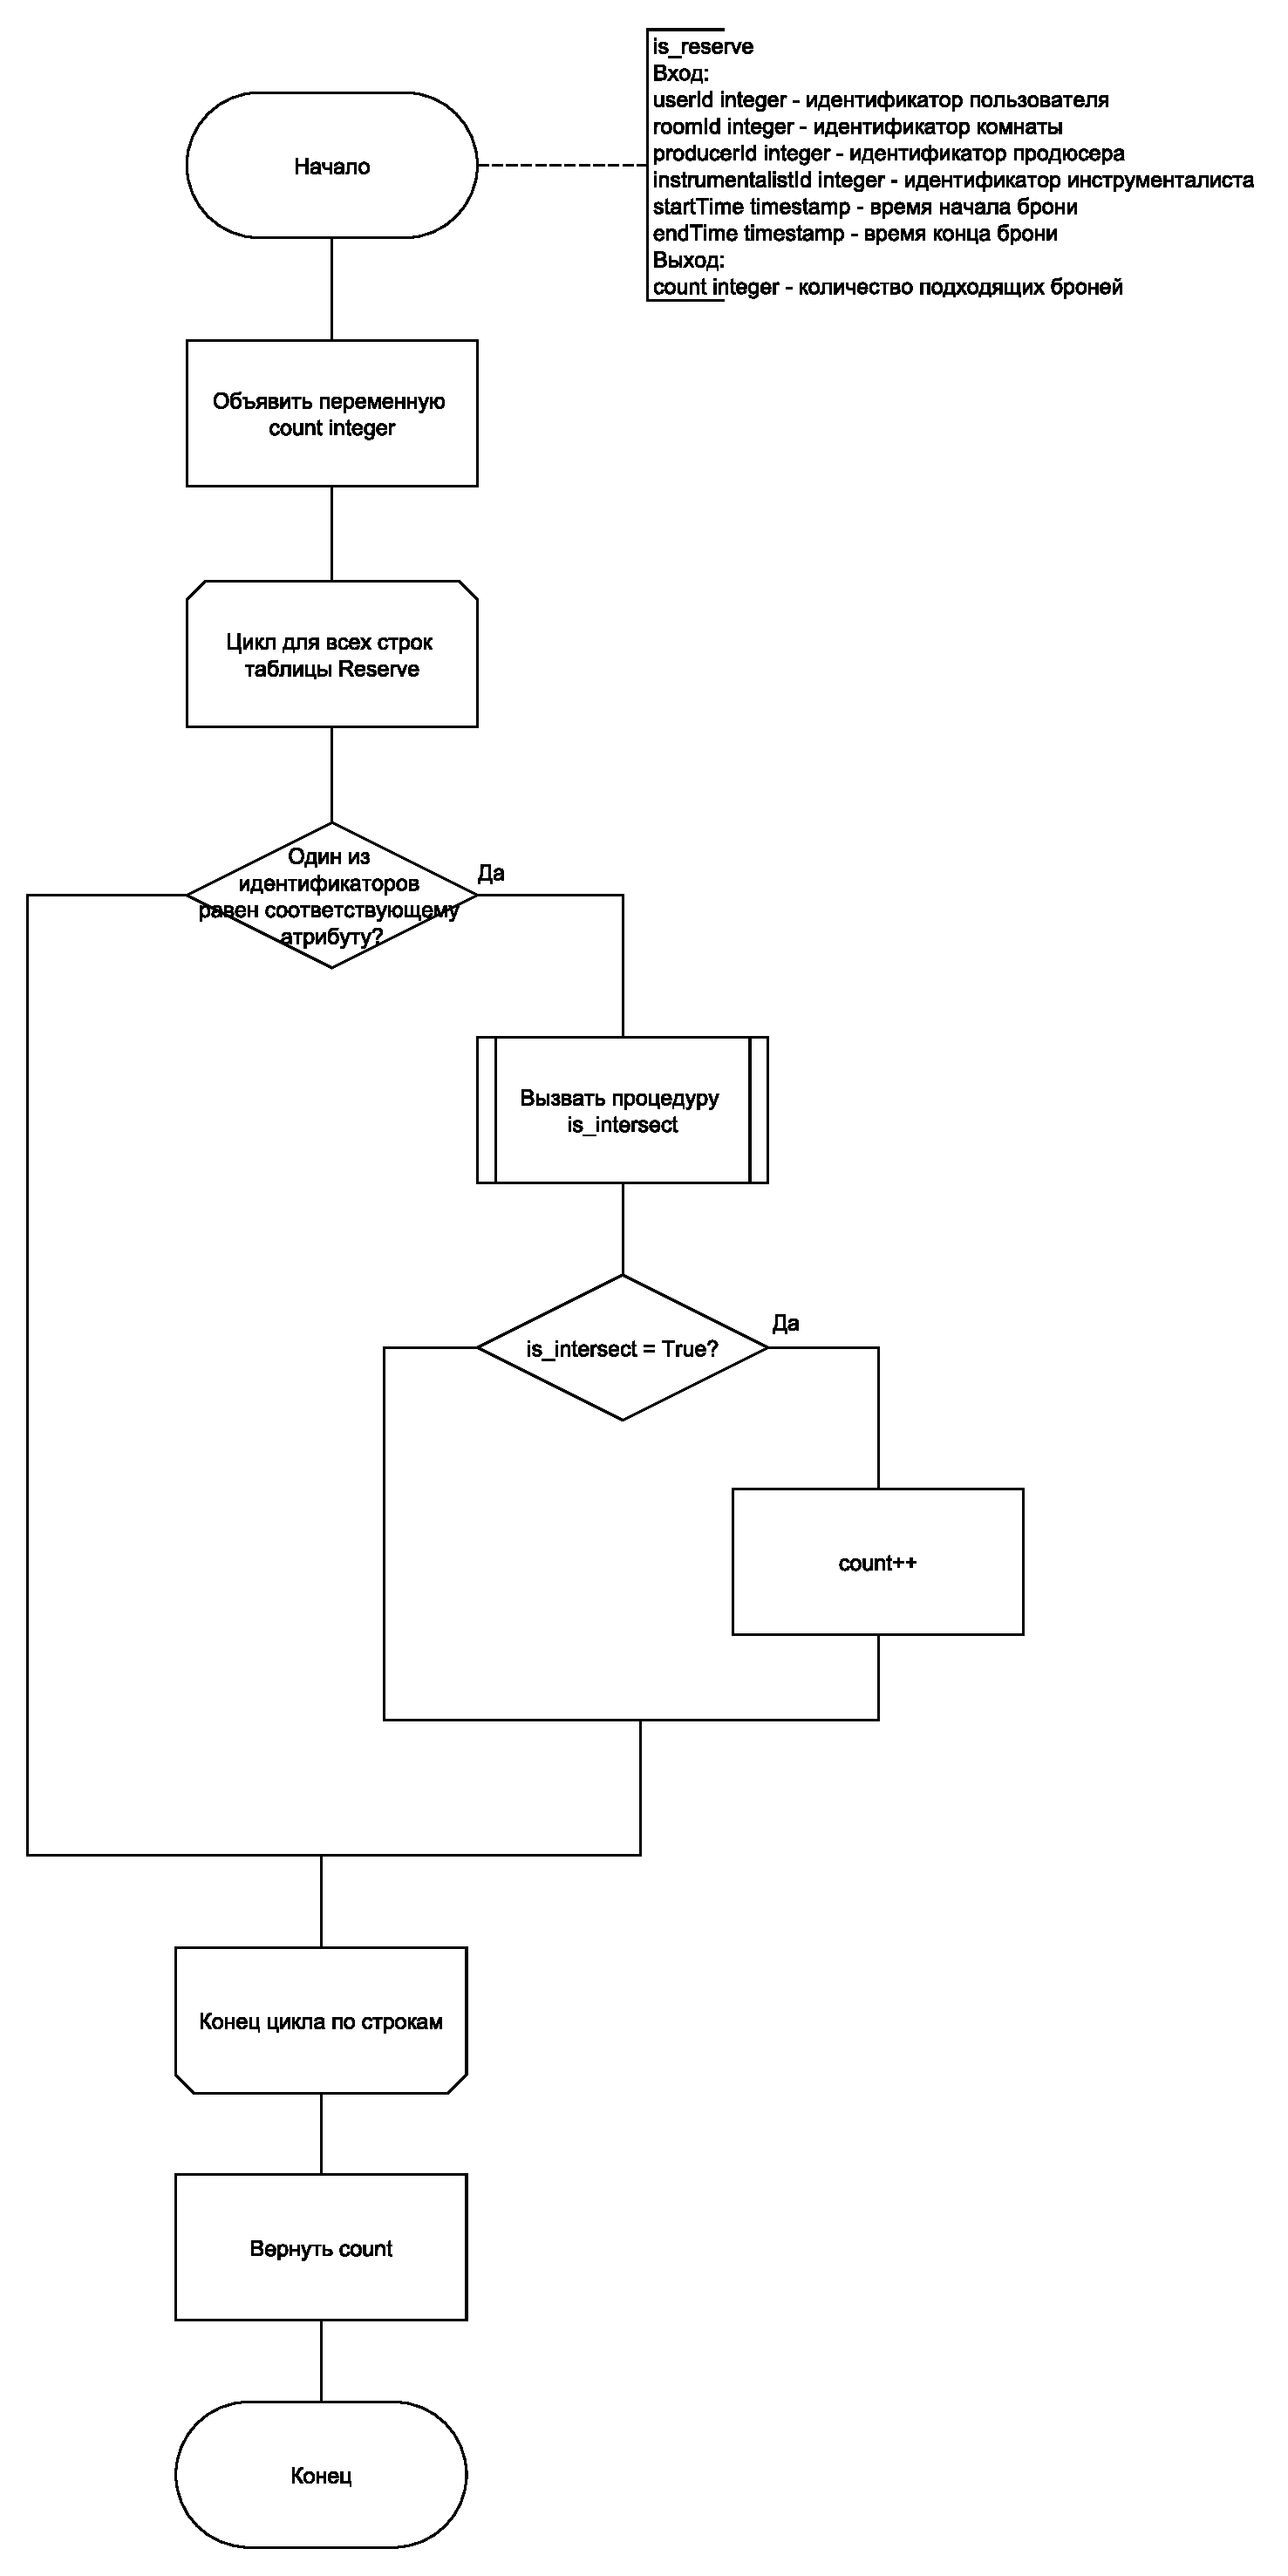
\includegraphics[height=0.95\textheight]{inc/img/is_reserve.pdf}
	\captionof{figure}{Алгоритм работы проверки занятости}
	\label{img:is_reserve}
\end{center}

\subsection{Процедура is\_intersect}
Данная процедура принимает 4 аргумента: выбранное пользователем начало времени, выбранный пользователем конец времени, время начала брони, время конца брони.
Если данные временные отрезки пересекаются, то процедура возвращает True, иначе --- False.

На рисунке \ref{img:is_reserve} представлен алгоритм работы проверки пересечения времени. 
\begin{center}
	\centering
	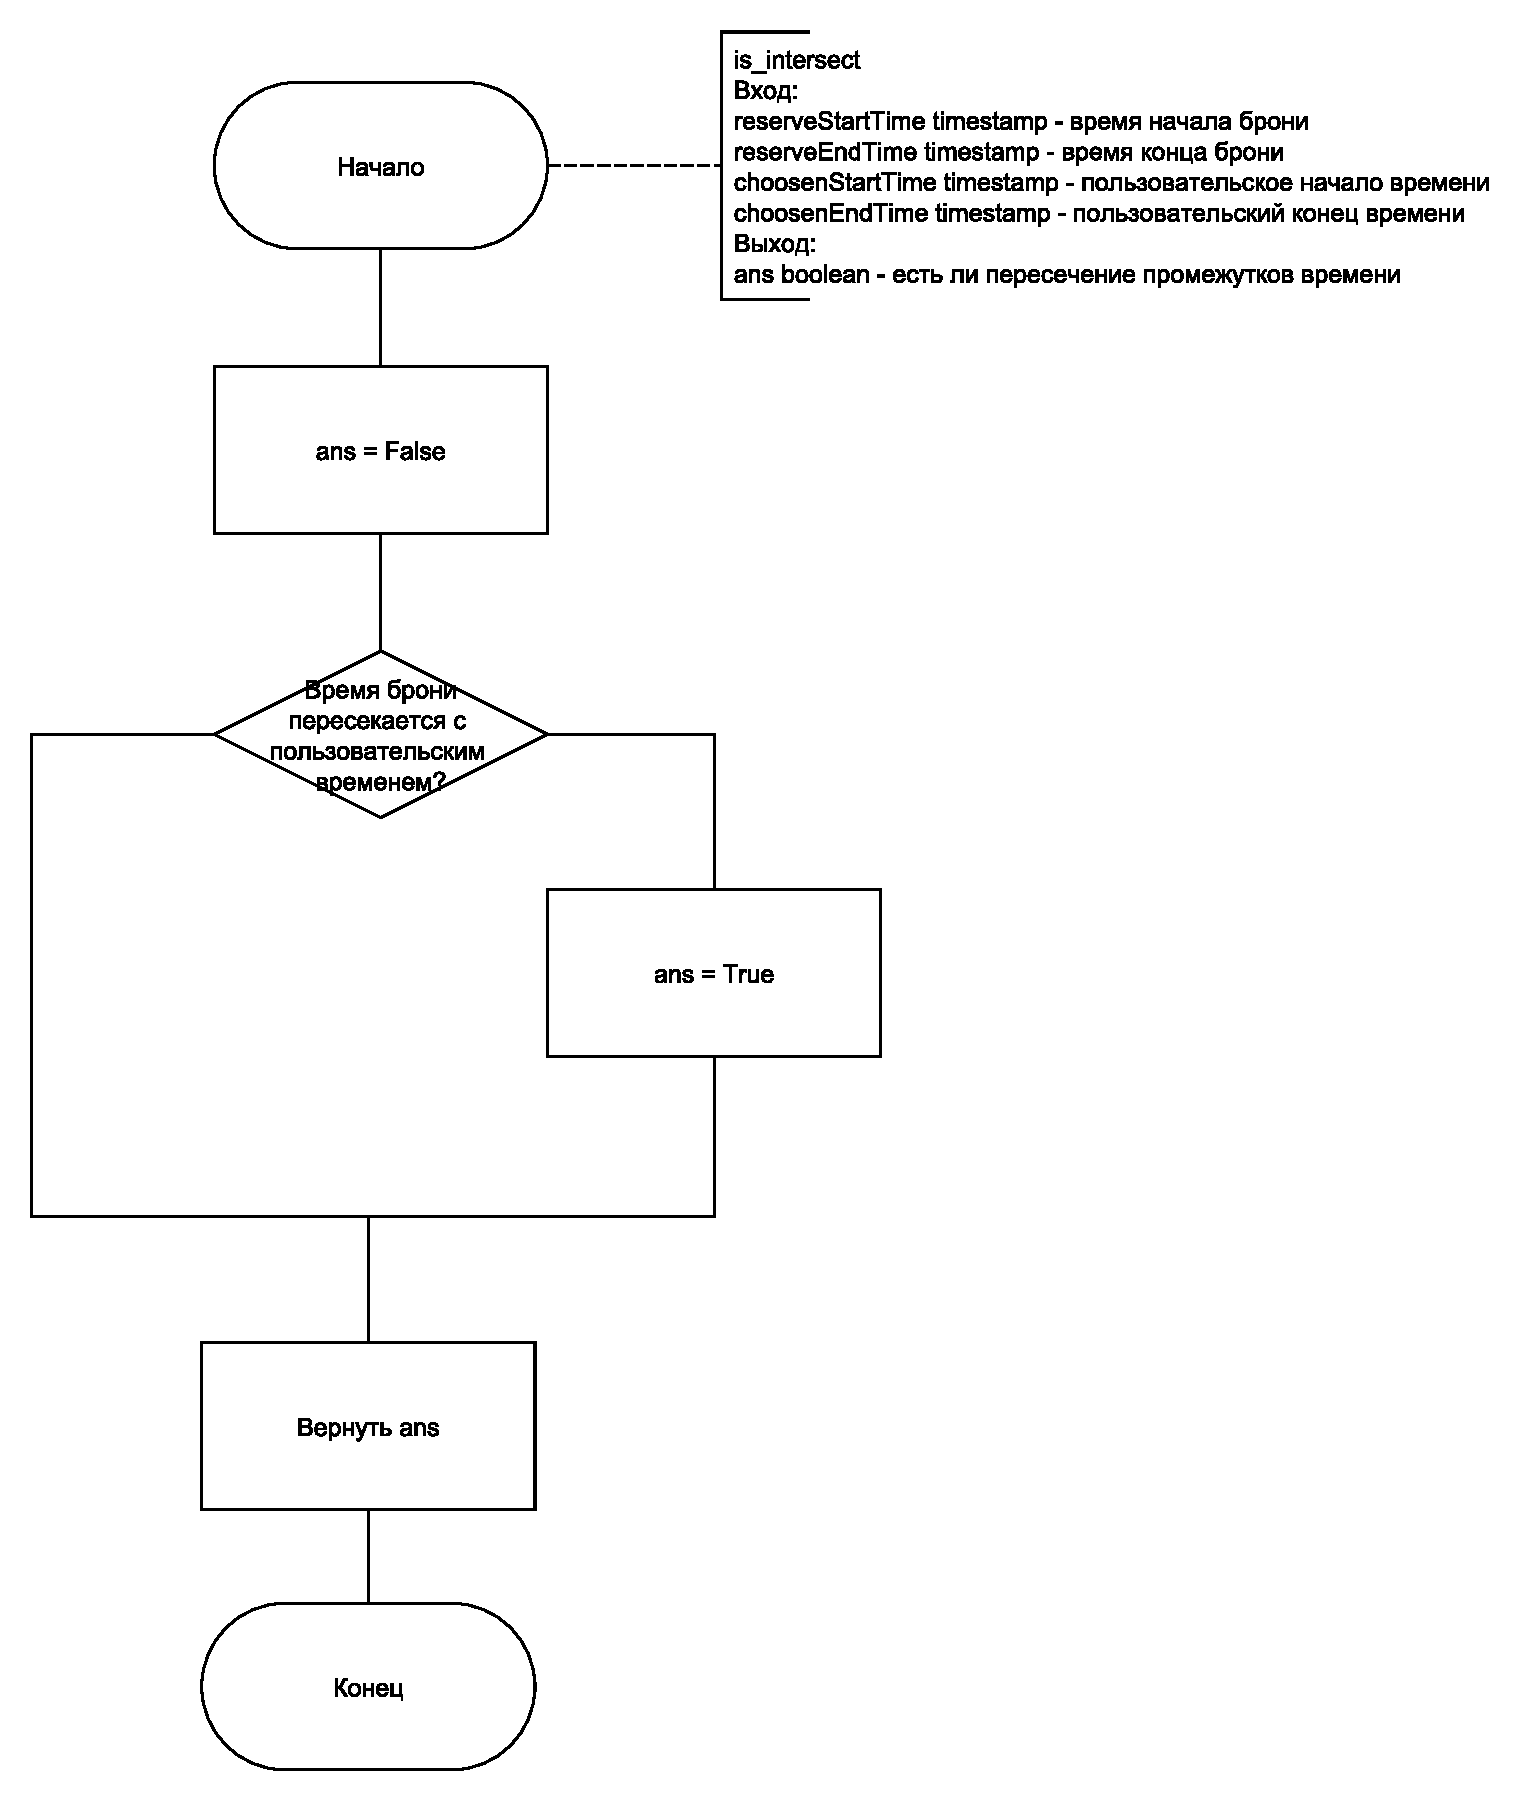
\includegraphics[height=0.65\textheight]{inc/img/is_intersect.pdf}
	\captionof{figure}{Алгоритм работы проверки пересечения времени}
	\label{img:is_intersect}
\end{center}

\section*{Вывод}

В данном разделе была представлена диаграмма проектируемой БД, описание сущностей, описание проектируемой ролевой модели и описание проектируемых процедур.


\chapter{Технологический раздел}
\section{Выбор СУБД}
\chapter{Исследовательский раздел}

В данном разделе будут представлены технические характеристики и будет проведено исследование.

\section{Технические характеристики}
Технические характеристики устройства, на котором выполнялось исследование:
\begin{itemize}
	\item операционная система: Ubuntu 20.04~\cite{ubuntu};
	\item размер оперативной памяти: 16 Гбайт;
	\item процессор AMD Ryzen 5 5500U with Radeon Graphics.

\end{itemize}
	
На протяжении всего тестирования компьютер был подключен к сети питания.
\section{Исследование}
Задача заключалась в исследования зависимости времени работы от сложности запроса.
Исследование проводилось на заранее заготовленной таблице, количество записей в которой было равно 500 штук.

Градация сложности запросов была следующая:
\begin{enumerate}
	\item запрос первой сложности:
		\begin{lstlisting}[language=sql, label=lst:query_1]
		select equipment.id from equipment\end{lstlisting}
	\item запрос второй сложности:
		\begin{lstlisting}[language=sql, label=lst:query_2]
		select equipment.id,
			equipment.name,
			equipment.type,
			equipment.studio_id
		from equipment\end{lstlisting}
	\item запрос третьей сложности:
		\begin{lstlisting}[language=sql, label=lst:query_2]
		select equipment.id,
			equipment.name,
			equipment.type,
			equipment.studio_id
		from equipment where 
			equipment.studio_id = $1\end{lstlisting}
	\item запрос четвертой сложности:
		\begin{lstlisting}[language=sql, label=lst:query_2]
		select equipment.id,
			equipment.name,
			equipment.type,
			equipment.studio_id
		from equipment where 
			equipment.studio_id = $1 and
			equipment.type = $2\end{lstlisting}
	\item запрос пятой сложности
			\begin{lstlisting}[language=sql, label=lst:query_2]
			select equipment.id,
				equipment.name,
				equipment.type,
				equipment.studio_id
			from equipment where 
				equipment.studio_id = $1 and
				equipment.type = $2 and 
				not exists
					(select * from reserved_equipments where equipment.id = reserved_equipments.equipment_id)\end{lstlisting}
	\item запрос шестой сложности
			\begin{lstlisting}[language=sql, label=lst:query_2]
			select equipment.id, 
				equipment.name,
				equipment.type,
				equipment.studio_id,
				to_char(reserve.start_time, 'YYYY-MM-DD HH24:MI:SS'),
				to_char(reserve.end_time, 'YYYY-MM-DD HH24:MI:SS')
			from equipment, reserve where 
				equipment.studio_id = $1 and 
				equipment.type = $2 and 
				exists 
					(select * from reserved_equipments where equipment.id = reserved_equipments.equipment_id)\end{lstlisting}
\end{enumerate}  

Для каждого запроса время замерялось 1000 раз и суммировалось.
После чего бралось среднее значение.

По итогам исследования получились следующие результаты, представленные в таблице~\ref{table:res} и на рисунке~\ref{img:chart}.

\begin{table}[h]

	\centering
	\begin{tabular}{ | c | c | }
		\hline
		Уровень сложности запроса & Время работы, мс \\ \hline
		1 & 1.181 \\
		2 & 1.383 \\
		3 & 1.397 \\
		4 & 1.402 \\
		5 & 1.445 \\
		6 & 1.532 \\
		\hline
	\end{tabular}
	\caption{Результаты исследования}
				\label{table:res}
\end{table}


\begin{center}
	\centering
	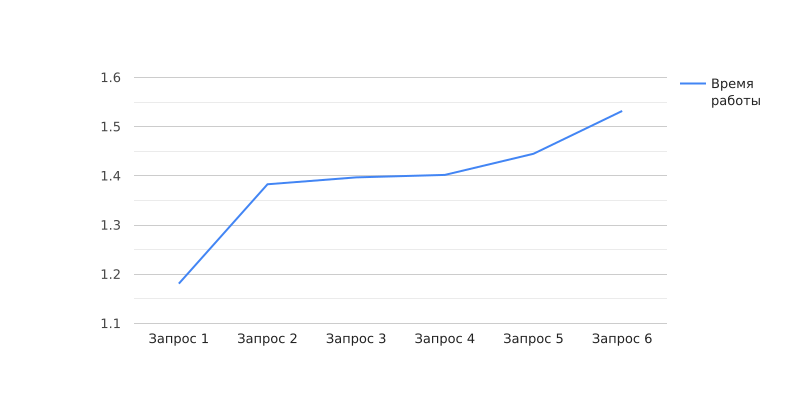
\includegraphics[height=0.3\textheight]{inc/img/chart.png}
	\captionof{figure}{График зависимости времени работы от сложности запроса}
	\label{img:chart}
\end{center}
\section*{Вывод}
В ходе выполнения исследовательской части было выявлено, что время работы напрямую зависит от сложности запроса --- чем сложнее запрос, тем больше времени системе требуется на его обработку.
Также на графике можно наблюдать довольно резкий скачок времени работы в 1.16 раз между Запросом 1 и Запросом 2.
Это можно объяснить тем, что в инструкции SELECT Запроса 1 необходимо вернуть одно значение, а в инструкции SELECT Запроса 2 4 значения.
При проходе по всей таблице, системе необходимо вернуть ответ, который будет включать в себя больше значений, чем при Запросе 1.
Также большое время при выполнении Запроса 6 можно объяснить работой с двумя таблицами.

 
\chapter*{ЗАКЛЮЧЕНИЕ}
\addcontentsline{toc}{chapter}{ЗАКЛЮЧЕНИЕ}

\makebibliography

\begin{appendices}
	\chapter{Тестирование БД}
	\begin{lstlisting}[language=go, label=lst:testing_code]
func TestStudioPostrgresql_Get(t *testing.T) {
type fields struct {
	db *pgxpool.Pool
}

type args struct {
	ctx     context.Context
	request *dto.GetStudioRequest
}

tests := []struct {
	name string
	args       args
	wantStudio *model.Studio
	wantErr    bool
}{
	{
		name: "test_pos_01",
		args: args{
			ctx: context.Background(),
			request: &dto.GetStudioRequest{
			Id: 1,
			},
		},
		wantStudio: &model.Studio{
			Id:   1,
			Name: "first",
		},
		wantErr: false,
	},
}

for _, tt := range tests {
	t.Run(tt.name, func(t *testing.T) {
		p := postgresql.NewStudioRepository(testDbInstance)

		gotStudio, err := p.Get(tt.args.ctx, tt.args.request)
		if (err != nil) != tt.wantErr {
			t.Errorf("Get() error = %v, wantErr %v", err, tt.wantErr)
		return
		}
		if !reflect.DeepEqual(gotStudio, tt.wantStudio) {
			t.Errorf("Get() gotStudio = %v, want %v", gotStudio, tt.wantStudio)
		}
	})
}
	\end{lstlisting}
	\captionof{figure}{Код тестирования}
\end{appendices}



\begin{lstlisting}[language=go, label=lst:testing_res]
=== RUN   TestEquipmentRepository_GetFullTimeFreeByStudioAndType
--- PASS: TestEquipmentRepository_GetFullTimeFreeByStudioAndType (0.01s)
=== RUN   TestEquipmentRepository_GetFullTimeFreeByStudioAndType/test_pos_01
	--- PASS: TestEquipmentRepository_GetFullTimeFreeByStudioAndType/test_pos_01 (0.01s)
=== RUN   TestEquipmentRepository_GetNotFullTimeFreeByStudioAndType
--- PASS: TestEquipmentRepository_GetNotFullTimeFreeByStudioAndType (0.01s)
=== RUN   TestEquipmentRepository_GetNotFullTimeFreeByStudioAndType/test_pos_01
	--- PASS: TestEquipmentRepository_GetNotFullTimeFreeByStudioAndType/test_pos_01 (0.01s)
=== RUN   TestReserveRepository_Add
--- PASS: TestReserveRepository_Add (0.00s)
=== RUN   TestReserveRepository_GetByRoomId
--- PASS: TestReserveRepository_GetByRoomId (0.01s)
=== RUN   TestReserveRepository_GetByRoomId/test_pos_01
	--- PASS: TestReserveRepository_GetByRoomId/test_pos_01 (0.01s)
=== RUN   TestReserveRepository_IsRoomReserve
--- PASS: TestReserveRepository_IsRoomReserve (0.00s)
=== RUN   TestReserveRepository_IsRoomReserve/test_pos_01
	--- PASS: TestReserveRepository_IsRoomReserve/test_pos_01 (0.00s)
=== RUN   TestReserveRepository_IsRoomReserve/test_pod_02
	--- PASS: TestReserveRepository_IsRoomReserve/test_pod_02 (0.00s)
=== RUN   TestReserveRepository_IsEquipmentReserve
--- PASS: TestReserveRepository_IsEquipmentReserve (0.00s)
=== RUN   TestReserveRepository_IsEquipmentReserve/test_pos_01
	--- PASS: TestReserveRepository_IsEquipmentReserve/test_pos_01 (0.00s)
=== RUN   TestRoomRepository_GetByStudio
--- PASS: TestRoomRepository_GetByStudio (0.00s)
=== RUN   TestRoomRepository_GetByStudio/test_pos_01
	--- PASS: TestRoomRepository_GetByStudio/test_pos_01 (0.00s)
=== RUN   TestStudioPostrgresql_Get
--- PASS: TestStudioPostrgresql_Get (0.00s)
=== RUN   TestStudioPostrgresql_Get/test_pos_01
	--- PASS: TestStudioPostrgresql_Get/test_pos_01 (0.00s)
=== RUN   TestStudioRepository_Update
--- PASS: TestStudioRepository_Update (0.04s)
=== RUN   TestStudioRepository_Update/test_pos_01
	--- PASS: TestStudioRepository_Update/test_pos_01 (0.04s)
=== RUN   TestStudioRepository_Add
--- PASS: TestStudioRepository_Add (0.11s)
=== RUN   TestStudioRepository_Add/test_pos_01
	--- PASS: TestStudioRepository_Add/test_pos_01 (0.11s)
=== RUN   TestStudioRepository_Delete
--- PASS: TestStudioRepository_Delete (0.02s)
=== RUN   TestStudioRepository_Delete/test_pos_01
	--- PASS: TestStudioRepository_Delete/test_pos_01 (0.02s)
=== RUN   TestUserRepository_GetByLogin
--- PASS: TestUserRepository_GetByLogin (0.01s)
=== RUN   TestUserRepository_GetByLogin/test_neg_01
	--- PASS: TestUserRepository_GetByLogin/test_neg_01 (0.01s)
PASS
\end{lstlisting}
\captionof{figure}{Результат тестирования}



\end{document}